\documentclass{article}

%%%%%%%%%%%%%%% LIBRERIAS %%%%%%%%%%%%%%%%%%%%%
\usepackage[thinc]{esdiff}
\usepackage{amsmath,amssymb}
\usepackage{caption}
\usepackage{titlesec}
\usepackage{titletoc}
\usepackage{graphicx}
\IfFileExists{spanish.ldf}
  {\usepackage[spanish,es-tabla]{babel}}
  {\usepackage[provide=*,spanish]{babel}}
\usepackage{icomma}
\usepackage{xurl}
\usepackage{hyperref}
\usepackage{float}
\usepackage[table]{xcolor}
\usepackage{circuitikz}
\usepackage[left=2cm, right=2cm, top=2cm, bottom=2cm, footskip=1cm]{geometry}
\usepackage{subcaption}
\usepackage{booktabs}
\usepackage{array}
\usepackage{longtable}
\usepackage{tabularx}
\usepackage{multirow}
\usepackage{enumitem}
\usepackage{setspace}
\usepackage{fancyhdr}
\usetikzlibrary{babel,arrows.meta,calc,positioning,decorations.pathmorphing}

%%%%%%%%%%%%%%%%%%% VARIABLES %%%%%%%%%%%%%%%%%%%%
\newcommand{\Facultad}{Instituto Tecnológico \\de\\ Buenos Aires}
\newcommand{\TPn}{Trabajo Práctico N° 3}
\newcommand{\TPtema}{Espectrometría gaseosa}
\graphicspath{{figuras/}}

%%%%%%%%%%%%%%%%%% FORMATO TÍTULO Y NUMERACIÓN %%%%%%%%%%%%%%%%%%%
\renewcommand{\thesection}{\arabic{section}.}
\renewcommand{\thesubsection}{\thesection\arabic{subsection}}
\setcounter{secnumdepth}{3}

\titleformat{\section}{\Large\bfseries}{\thesection}{1em}{}
\titleformat{\subsection}{\large\bfseries}{\thesubsection}{0.5em}{}
\titleformat{\subsubsection}{\normalsize\bfseries}{\thesubsubsection}{0.5em}{}

%%%%%%%%%%%%%%% SOPORTE DEL CUERPO DEL INFORME %%%%%%%%%%%%%%%%%%%%%
\definecolor{azulencabezado}{HTML}{163A5F}
\definecolor{rojoref}{HTML}{B03A2E}
\newcolumntype{Y}{>{\raggedright\arraybackslash}X}
\newcolumntype{C}[1]{>{\centering\arraybackslash}p{#1}}
\newcolumntype{L}[1]{>{\raggedright\arraybackslash}p{#1}}
\newcommand{\nm}{\ \mathrm{nm}}

\hypersetup{
  hidelinks,
  pdftitle={Informe del experimento de Espectrometría gaseosa},
  pdfsubject={Laboratorio de Física IV},
  pdfkeywords={Espectrometría, líneas espectrales, Balmer, laboratorio, Física IV}
}

\makeatletter
\providecommand{\ttl@finishall}{}
\makeatother

%%%%%%%%%%%%%%%%%%% ARCHIVO %%%%%%%%%%%%%%%%%%%%%%%%
\begin{document}
\renewcommand{\tablename}{Tabla}
\hypersetup{pageanchor=false}

%%%CARATULA%%%
\begin{titlepage}

        \begin{flushleft}
            \centering
            
\includegraphics[width=0.3\textwidth]{Logo_ITBA.png}
        \end{flushleft}

        \centering

        {\scshape\LARGE \Facultad\par}
        \vspace{1cm}

        {\huge\bfseries \TPn\par}
        \vspace{1.5cm}
        {\Large Laboratorio de Física IV\\ 93.61 \par}
        \vspace{0.5cm}
        {\Large \TPtema\par}
        \vspace{0.5cm}
        {\large Docente a cargo: Raúl Florentino\par}
        \vfill
        {\Large \bfseries Grupo N° 55 \par}
        \vspace{1cm}
        {\large Juan Ignacio Fogolin Lagares \hfill Legajo: 66409  \par}
        {\large Rita Moschini \hfill Legajo: 67026 \par}
        {\large Agustín Alejandro Montoto \hfill Legajo: 65511\par}
        \vfill
        {\large Fecha de entrega: \today\par}
        \vfill

        \begin{flushleft}
        \renewcommand{\arraystretch}{2.2}
        \begin{tabularx}{\textwidth}{@{}L{8.5cm}Y@{}}
            \toprule
            \textbf{Fecha de aprobación:} & \\
            \midrule
            \textbf{Comentarios y observaciones del docente:} & \\
             & \\
             & \\
            \bottomrule
        \end{tabularx}
        \end{flushleft}

\end{titlepage}

\pagenumbering{gobble}
\tableofcontents
\newpage

%%%%%%%%%%%%%%%%%%% CUERPO DEL INFORME %%%%%%%%%%%%%%%%%%%%%%%%
\pagenumbering{arabic}
\setcounter{page}{1}
\hypersetup{pageanchor=true}

\setstretch{1.12}
\setlength{\parindent}{0.7cm}
\setlength{\parskip}{0.25em}
\setlength{\arrayrulewidth}{0.45pt}
\setlength{\tabcolsep}{5pt}
\arrayrulecolor{black}
\renewcommand{\arraystretch}{1.22}

\renewcommand{\thesection}{\arabic{section}}
\renewcommand{\thesubsection}{\thesection.\arabic{subsection}}
\renewcommand{\thesubsubsection}{\thesubsection.\arabic{subsubsection}}
\setcounter{secnumdepth}{3}

\titleformat{\section}{\Large\bfseries\color{black}}{\thesection}{0.6em}{}
\titleformat{\subsection}{\large\bfseries\color{black}}{\thesubsection}{0.55em}{}
\titlespacing*{\section}{0pt}{1.1em}{0.45em}
\titlespacing*{\subsection}{0pt}{0.9em}{0.35em}
\titlespacing*{\subsubsection}{0pt}{0.8em}{0.3em}

\captionsetup{font={small,it},labelfont=it,justification=centering}
\setlist[itemize]{leftmargin=1.05cm,itemsep=0.18em,topsep=0.25em}
\setlist[enumerate]{leftmargin=1.05cm,itemsep=0.22em,topsep=0.25em}

\pagestyle{fancy}
\fancyhf{}
\fancyhead[L]{\small\itshape{} Laboratorio de Física IV\/}
\fancyhead[R]{\small\itshape{} Instituto Tecnológico de Buenos Aires\/}
\fancyfoot[C]{\thepage}
\renewcommand{\headrulewidth}{0pt}
\renewcommand{\footrulewidth}{0pt}

%=====================================================================
\section{Objetivos y resumen}

\subsection{Objetivos}

\begin{itemize}
    \item Estudiar el espectro de emisión de distintos gases excitados eléctricamente en tubos de Plücker, midiendo la longitud de onda de sus líneas con un espectrómetro de red de difracción.
    \item Comparar las líneas medidas para helio, kriptón y mercurio con valores de referencia de bases de datos reconocidas (NIST) y cuantificar el error porcentual de cada medición.
    \item Determinar el contenido de tres tubos incógnita a partir de su espectro de emisión.
    \item Aplicar las fórmulas de Balmer y de Lyman para calcular las líneas del espectro del hidrógeno y compararlas con el espectro obtenido.
\end{itemize}

\subsection{Resumen}

Cada elemento químico emite luz únicamente en un conjunto discreto de longitudes de onda, determinado por la estructura de sus niveles de energía; su espectro de líneas funciona, por lo tanto, como una huella digital que permite identificarlo. En esta práctica se excitaron eléctricamente distintos gases contenidos en tubos de Plücker mediante una fuente de alta tensión. La radiación emitida se condujo mediante una fibra óptica hasta un espectrómetro de red de difracción, y con el software de adquisición se midió la longitud de onda $\lambda$ del máximo de cada línea junto con su ancho de banda $\Delta\lambda$.

Para los tres gases conocidos (He, Kr y Hg) se registraron doce líneas, que se compararon con las tablas de líneas intensas del NIST. Se verificó además que las líneas del infrarrojo cercano medidas en el tubo de kriptón pertenecen efectivamente al Kr~I, mientras que las dos líneas del tubo de mercurio que no corresponden al Hg coinciden con dos de las líneas más intensas del argón (Ar~I), presente en el tubo como gas de llenado. Luego se analizaron los espectros de tres tubos incógnita: uno resultó ser neón (17 líneas identificadas), otro hidrógeno (líneas de la serie de Balmer) y el tercero no presenta un espectro atómico, sino una banda ancha propia de una fuente de estado sólido tipo LED. Finalmente, se calcularon las series de Balmer y de Lyman y, a partir de las líneas H$\alpha$ y H$\beta$ medidas, se obtuvo un valor experimental de la constante de Rydberg.

\textbf{Resultados principales:} las 12 líneas de los gases conocidos difieren de los valores del NIST en menos de $0,9\nm$ (error porcentual máximo de $0,12\%$), siempre dentro de la incertidumbre $\Delta\lambda$ del instrumento. Los tubos incógnita N.º 2 y N.º 3 contienen neón e hidrógeno, respectivamente, y el N.º 1 corresponde a una fuente no atómica de banda ancha centrada en $585\nm$. La constante de Rydberg experimental resultó $R_{\mathrm{exp}}=(1,0978\pm0,0027)\times10^{7}\ \mathrm{m^{-1}}$, a un $0,09\%$ del valor teórico.

%=====================================================================
\section{Introducción teórica}

\subsection{Espectros atómicos de emisión}

Según la mecánica cuántica, un electrón ligado a un átomo solo puede ocupar estados con energías discretas $E_1<E_2<E_3<\dots$ Cuando el átomo, previamente excitado a un nivel $E_i$, decae espontáneamente a un nivel inferior $E_f$, emite un fotón cuya energía es exactamente la diferencia entre ambos niveles:
\begin{equation}
    h\nu = \frac{hc}{\lambda} = E_i-E_f
    \qquad\Longrightarrow\qquad
    \lambda=\frac{hc}{E_i-E_f},
    \label{eq:foton}
\end{equation}
donde $h$ es la constante de Planck y $c$ la velocidad de la luz. Como los niveles de energía dependen de la carga nuclear y de la interacción entre los electrones, cada elemento posee un conjunto propio de longitudes de onda de emisión. No todas las transiciones son igualmente probables (reglas de selección), por lo que las líneas tienen intensidades muy distintas entre sí.

En un tubo de Plücker el gas se encuentra a baja presión entre dos electrodos. Al aplicar una tensión del orden de los kilovoltios, los pocos electrones libres presentes se aceleran, ionizan nuevos átomos y producen una descarga autosostenida. En los choques inelásticos de los electrones con los átomos estos quedan en estados excitados, que decaen emitiendo radiación. A baja presión los átomos están prácticamente aislados, por lo que el espectro es de líneas finas y bien separadas, a diferencia del espectro continuo de un sólido incandescente.

\subsection{El átomo de hidrógeno: series de Lyman y Balmer}

El hidrógeno es el único átomo neutro cuyos niveles pueden calcularse de forma exacta y sencilla. El modelo de Bohr, y luego la ecuación de Schrödinger, conducen a \cite{eisberg}
\begin{equation}
    E_n=-\frac{hc\,R_H}{n^2}\approx-\frac{13,6\ \mathrm{eV}}{n^2},\qquad n=1,2,3,\dots
    \label{eq:niveles}
\end{equation}
Combinando las ecuaciones \eqref{eq:foton} y \eqref{eq:niveles} se obtiene la fórmula de Rydberg para la transición $n_i\to n_f$:
\begin{equation}
    \frac{1}{\lambda}=R_H\left(\frac{1}{n_f^2}-\frac{1}{n_i^2}\right),\qquad n_i>n_f.
    \label{eq:rydberg}
\end{equation}
Las transiciones que terminan en un mismo nivel forman una \emph{serie}: la serie de \textbf{Lyman} ($n_f=1$) cae en el ultravioleta lejano, la de \textbf{Balmer} ($n_f=2$) en el visible y ultravioleta cercano, y la de Paschen ($n_f=3$) en el infrarrojo (Figura~\ref{fig:niveles}). Las líneas de Balmer se designan H$\alpha$ ($3\to2$), H$\beta$ ($4\to2$), H$\gamma$ ($5\to2$), etc. Balmer encontró empíricamente en 1885 que estas líneas cumplen $\lambda=B\,n^2/(n^2-4)$ con $B\approx364,6\nm$, que es precisamente el caso $n_f=2$ de la ecuación \eqref{eq:rydberg} con $B=4/R_H$.

La constante $R_H$ difiere levemente de la constante de Rydberg $R_\infty$ porque el núcleo no es infinitamente pesado: el electrón y el protón giran en torno al centro de masa, lo que se tiene en cuenta reemplazando la masa del electrón por la masa reducida,
\begin{equation}
    R_H=\frac{R_\infty}{1+m_e/m_p}=1,0967758\times10^{7}\ \mathrm{m^{-1}},
    \label{eq:RH}
\end{equation}
con $R_\infty=1,0973731568\times10^{7}\ \mathrm{m^{-1}}$ y $m_p/m_e=1836,15267$ (CODATA 2018 \cite{codata}).

\begin{figure}[H]
\centering
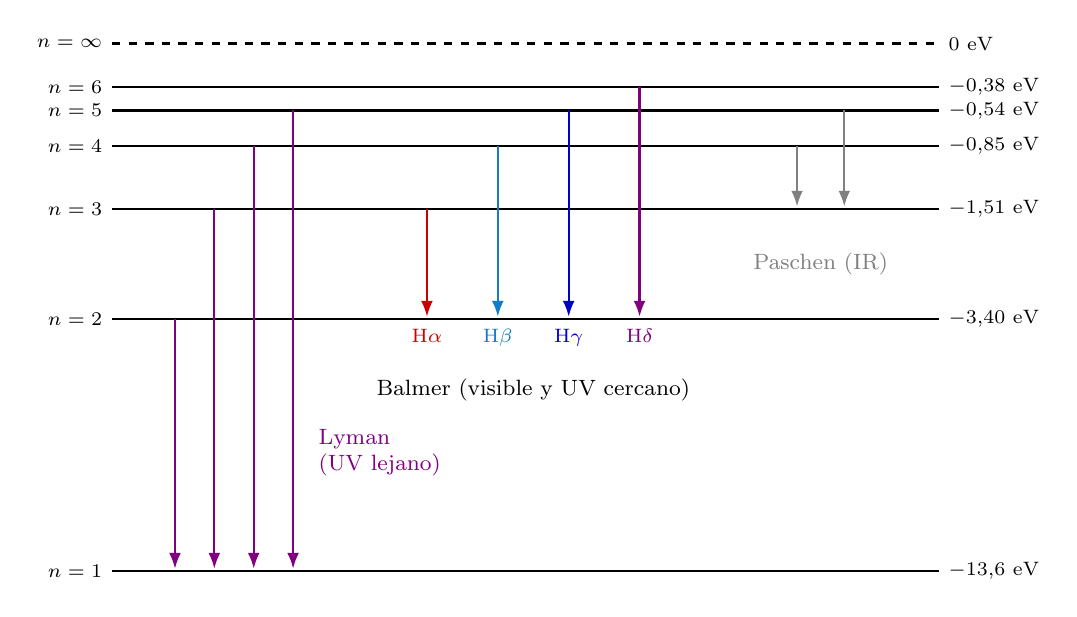
\begin{tikzpicture}[x=1cm,y=1cm,>={Latex[length=2mm]},font=\small]
    % altura esquemática (no proporcional) de cada nivel
    \foreach \n/\y/\E in {1/0/{-13,6},2/3.2/{-3,40},3/4.6/{-1,51},4/5.4/{-0,85},5/5.85/{-0,54},6/6.15/{-0,38}}{
        \draw[thick] (0,\y) -- (10.5,\y);
        \node[left,font=\scriptsize] at (0,\y) {$n=\n$};
        \node[right,font=\scriptsize] at (10.5,\y) {$\E$ eV};
    }
    \draw[thick,dashed] (0,6.7) -- (10.5,6.7);
    \node[left,font=\scriptsize] at (0,6.7) {$n=\infty$};
    \node[right,font=\scriptsize] at (10.5,6.7) {$0$ eV};
    % Lyman
    \foreach \y/\x in {3.2/0.8,4.6/1.3,5.4/1.8,5.85/2.3}{
        \draw[->,violet,thick] (\x,\y) -- (\x,0.03);
    }
    \node[violet,align=left,font=\footnotesize,anchor=west] at (2.5,1.5) {Lyman\\(UV lejano)};
    % Balmer
    \foreach \y/\x/\c/\nom in {4.6/4.0/red!80!black/H$\alpha$,5.4/4.9/cyan!60!blue/H$\beta$,5.85/5.8/blue!80!black/H$\gamma$,6.15/6.7/violet/H$\delta$}{
        \draw[->,\c,thick] (\x,\y) -- (\x,3.23);
        \node[\c,below,font=\scriptsize] at (\x,3.2) {\nom};
    }
    \node[align=center,font=\footnotesize] at (5.35,2.3) {Balmer (visible y UV cercano)};
    % Paschen
    \foreach \y/\x in {5.4/8.7,5.85/9.3}{
        \draw[->,gray,thick] (\x,\y) -- (\x,4.63);
    }
    \node[gray,align=center,font=\footnotesize] at (9.0,3.9) {Paschen (IR)};
\end{tikzpicture}
\caption{Niveles de energía del hidrógeno (escala vertical esquemática, no proporcional) y primeras transiciones de las series de Lyman, Balmer y Paschen.}
\label{fig:niveles}
\end{figure}

\textbf{Longitudes de onda en aire y en vacío.} La ecuación \eqref{eq:rydberg} da la longitud de onda en el vacío. El espectrómetro, en cambio, mide en aire, cuyo índice de refracción $n_{\mathrm{aire}}\approx1,00028$ reduce la longitud de onda a $\lambda_{\mathrm{aire}}=\lambda_{\mathrm{vac}}/n_{\mathrm{aire}}$ (unos $0,18\nm$ para H$\alpha$). Por convención, las tablas del NIST informan longitudes de onda en aire por encima de $200\nm$ \cite{nist-handbook}, de modo que la comparación se realiza en aire; para el índice del aire se utilizó la fórmula de Edlén en la forma dada por Morton \cite{morton}.

\subsection{Espectrómetro de red de difracción}

Una red de difracción es una superficie con un gran número de surcos paralelos separados una distancia $d$. La luz difractada por los distintos surcos interfiere constructivamente solo en las direcciones $\theta_m$ que satisfacen la ecuación de la red \cite{hecht},
\begin{equation}
    d\,(\sin\theta_i+\sin\theta_m)=m\,\lambda,\qquad m=0,\pm1,\pm2,\dots
    \label{eq:red}
\end{equation}
donde $\theta_i$ es el ángulo de incidencia y $m$ el orden de difracción. Para $m\neq0$ cada longitud de onda sale en una dirección distinta: la red \emph{dispersa} la luz. En un espectrómetro compacto como el utilizado, la luz ingresa por una rendija, es colimada por un espejo, dispersada por una red fija y enfocada sobre un detector lineal (CCD). Cada píxel del detector corresponde a una longitud de onda según una calibración polinómica almacenada en el equipo, y el software muestra la intensidad (en cuentas) en función de $\lambda$.

La resolución está limitada por el ancho de la rendija y el tamaño de los píxeles; para este equipo resulta del orden de $1$ a $2\nm$. De la ecuación \eqref{eq:red} se desprende además que la luz de longitud de onda $\lambda$ difractada en segundo orden ($m=2$) llega al mismo lugar que la de $2\lambda$ en primer orden, lo que puede generar líneas espurias si el equipo no dispone de un filtro separador de órdenes.

\subsection{Ancho de las líneas: fuentes atómicas y de estado sólido}

Las líneas atómicas tienen un ancho intrínseco extremadamente pequeño. El ensanchamiento natural es del orden de $10^{-5}\nm$ y el ensanchamiento Doppler, debido a la agitación térmica, vale
\begin{equation}
    \frac{\Delta\lambda_D}{\lambda}=\sqrt{\frac{8k_BT\ln2}{Mc^2}},
\end{equation}
que para el hidrógeno a temperatura ambiente da $\Delta\lambda_D\approx0,01\nm$ en H$\alpha$. En consecuencia, el ancho observado de cualquier línea atómica está dominado por la resolución del instrumento ($\sim2\nm$).

La situación es muy distinta en un diodo emisor de luz (LED). Allí los fotones se emiten al recombinarse electrones de la banda de conducción con huecos de la banda de valencia, y como ambos portadores tienen una distribución térmica de energías, el espectro es una banda cuyo ancho a media altura es aproximadamente $\Delta E\approx1,8\,k_BT\approx46\ \mathrm{meV}$ a $300$~K \cite{schubert}. En longitud de onda,
\begin{equation}
    \Delta\lambda\approx\frac{\lambda^2}{hc}\,\Delta E,
    \label{eq:anchoLED}
\end{equation}
lo que equivale a unos $13\nm$ para $\lambda\approx585\nm$. El ancho de la emisión permite entonces distinguir con claridad una fuente atómica (líneas de ancho instrumental) de una fuente de estado sólido (banda de decenas de nanómetros).

%=====================================================================
\section{Instrumentos y elementos empleados}

\begin{longtable}{@{}L{4.2cm}L{6.6cm}L{5.4cm}@{}}
    \caption{Instrumentos y elementos del montaje experimental.}\label{tab:instrumentos}\\
    \toprule
    \textbf{Elemento} & \textbf{Función} & \textbf{Especificación relevante} \\
    \midrule
    \endfirsthead
    \toprule
    \textbf{Elemento} & \textbf{Función} & \textbf{Especificación relevante} \\
    \midrule
    \endhead
    \bottomrule
    \endfoot
    Fuente de alta tensión & Produce la descarga eléctrica que excita el gas del tubo. & Tensión del orden de los kV \\
    Tubos de Plücker & Contienen el gas a baja presión entre dos electrodos. & He, Kr, Hg e incógnitas N.º 1, 2 y 3 \\
    Fibra óptica & Conduce la radiación desde el tubo hasta la rendija del espectrómetro. & Posición ajustable para evitar la saturación \\
    Espectrómetro de red de difracción & Dispersa la radiación y mide su intensidad en función de $\lambda$. & Rango de $350$ a $1000\nm$; resolución $\approx2\nm$ \\
    PC con software de adquisición & Visualiza el espectro y permite leer $\lambda$ y el ancho de banda con un cursor. & Intensidad en cuentas (máx. $\approx4000$) \\
\end{longtable}

\begin{figure}[H]
\centering
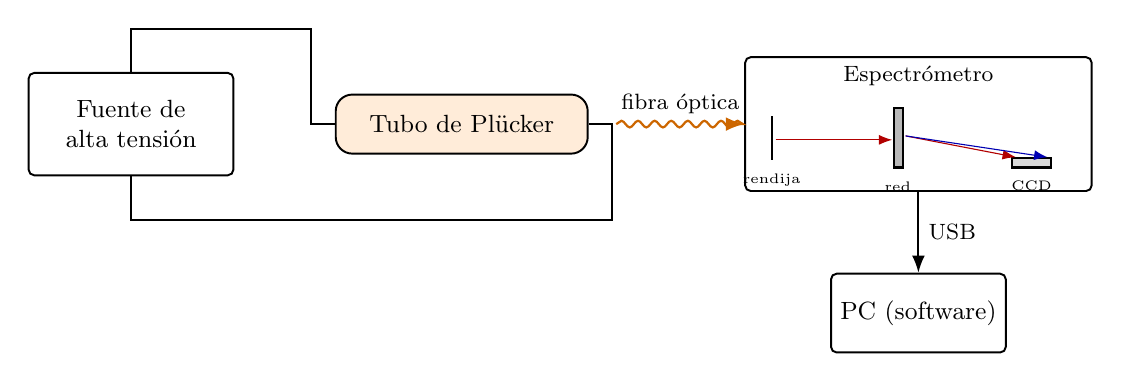
\begin{tikzpicture}[font=\small,>=Latex,line width=.7pt]
    \node[draw,rounded corners=2pt,minimum width=2.6cm,minimum height=1.3cm,align=center] (hv) at (0,0) {Fuente de\\alta tensión};
    \node[draw,rounded corners=6pt,minimum width=3.2cm,minimum height=0.75cm,fill=orange!15,align=center] (tubo) at (4.2,0) {Tubo de Plücker};
    \draw (hv.north) -- ++(0,0.55) -| ([xshift=-0.3cm]tubo.west) -- (tubo.west);
    \draw (hv.south) -- ++(0,-0.55) -| ([xshift=0.3cm]tubo.east) -- (tubo.east);
    \node[draw,rounded corners=2pt,minimum width=4.4cm,minimum height=1.7cm,align=center] (esp) at (10.0,0) {};
    \node[font=\footnotesize,anchor=north] at (esp.north) {Espectrómetro};
    \draw[thick] ([xshift=0.35cm,yshift=-0.45cm]esp.west) -- ++(0,0.55);
    \node[font=\tiny,anchor=north] at ([xshift=0.35cm,yshift=-0.5cm]esp.west) {rendija};
    \draw[thick,fill=gray!55] ([xshift=1.9cm,yshift=-0.55cm]esp.west) rectangle ++(0.12,0.75);
    \node[font=\tiny,anchor=north] at ([xshift=1.95cm,yshift=-0.6cm]esp.west) {red};
    \draw[thick,fill=gray!30] ([xshift=3.4cm,yshift=-0.55cm]esp.west) rectangle ++(0.5,0.12);
    \node[font=\tiny,anchor=north] at ([xshift=3.65cm,yshift=-0.6cm]esp.west) {CCD};
    \draw[->,thin,red!70!black] ([xshift=0.4cm,yshift=-0.2cm]esp.west) -- ([xshift=1.88cm,yshift=-0.2cm]esp.west);
    \draw[->,thin,red!70!black] ([xshift=2.05cm,yshift=-0.15cm]esp.west) -- ([xshift=3.45cm,yshift=-0.42cm]esp.west);
    \draw[->,thin,blue!70!black] ([xshift=2.05cm,yshift=-0.15cm]esp.west) -- ([xshift=3.85cm,yshift=-0.42cm]esp.west);
    \draw[->,decorate,decoration={snake,amplitude=1.2pt,segment length=6pt},orange!80!black,thick] (tubo.east) ++(0.35,0) -- node[above,black,font=\footnotesize]{fibra óptica} (esp.west);
    \node[draw,rounded corners=2pt,minimum width=2.2cm,minimum height=1.0cm,align=center] (pc) at (10.0,-2.4) {PC (software)};
    \draw[->] (esp.south) -- node[right,font=\footnotesize]{USB} (pc.north);
\end{tikzpicture}
\caption{Esquema del montaje: la descarga en el tubo emite luz que la fibra óptica lleva al espectrómetro; la red dispersa cada longitud de onda hacia un píxel distinto del detector.}
\label{fig:montaje}
\end{figure}

%=====================================================================
\section{Procedimiento experimental}

Se siguió el procedimiento indicado en la guía de la cátedra \cite{consigna}:

\begin{enumerate}
    \item Se colocó el tubo de Plücker en el soporte de la fuente de alta tensión y se encendió la descarga, evitando tocar los contactos mientras el tubo estaba energizado.
    \item Se posicionó el extremo de la fibra óptica frente al tubo y se ajustó su distancia y orientación para obtener el mayor flujo de radiación sin saturar el detector.
    \item En el software del espectrómetro se ajustaron el tiempo de integración y el promediado hasta observar con claridad el espectro de emisión.
    \item Con el cursor del programa se midió la longitud de onda $\lambda$ del máximo de cada línea y su ancho de banda $\Delta\lambda$, y se registró el color observado.
    \item Se repitió el procedimiento con los tubos de He, Kr y Hg y luego con los tres tubos incógnita, cuyos espectros completos se guardaron como capturas de pantalla (Anexo~\ref{anexo}).
\end{enumerate}

%=====================================================================
\section{Datos obtenidos, discusión y cálculo de errores}

\subsection{Tratamiento de incertidumbres}

Para cada línea se adoptó como incertidumbre de la longitud de onda el ancho de banda $\Delta\lambda$ leído en el software ($1,5$ a $2,5\nm$), que refleja la resolución del espectrómetro y la imprecisión al ubicar el máximo con el cursor. Como medida de exactitud se utilizó, según la consigna, el error porcentual respecto del valor de referencia:
\begin{equation}
    \varepsilon_{\%}=\frac{\left|\lambda_{\mathrm{med}}-\lambda_{\mathrm{ref}}\right|}{\lambda_{\mathrm{ref}}}\times100\%.
    \label{eq:error}
\end{equation}
Se consideró que una medición es compatible con el valor de referencia si $|\lambda_{\mathrm{med}}-\lambda_{\mathrm{ref}}|\le\Delta\lambda$. Los valores de referencia son las longitudes de onda en aire de las tablas de líneas intensas del \emph{Handbook of Basic Atomic Spectroscopic Data} del NIST \cite{nist-handbook}, citadas individualmente en cada caso.

\subsection{Gases conocidos: helio, kriptón y mercurio}

La Tabla~\ref{tab:conocidos} reúne las doce líneas medidas, en el formato pedido por la consigna, junto con la línea del NIST a la que corresponden y la especie que la emite.

\begin{table}[H]
\centering\small
\caption{Líneas medidas para los gases conocidos y comparación con el NIST (longitudes de onda en aire) \cite{nist-he,nist-kr,nist-hg,nist-ar}.}
\label{tab:conocidos}
\begin{tabular}{@{}llccccrc@{}}
\toprule
\textbf{Elemento} & \textbf{Color} & $\boldsymbol{\lambda}$ \textbf{(nm)} & $\boldsymbol{\Delta\lambda}$ \textbf{(nm)} & \textbf{Valor real (nm)} & \textbf{Especie} & $\boldsymbol{\lambda-\lambda_{\mathrm{ref}}}$ \textbf{(nm)} & \textbf{Error (\%)}\\
\midrule
\multirow{4}{*}{Helio}    & Verde         & 501,0 & 2,0 & 501,57 & He I & $-0,57$ & 0,114\\
                          & Amarillo      & 587,0 & 2,0 & 587,56 & He I & $-0,56$ & 0,095\\
                          & Rojo          & 668,0 & 2,0 & 667,82 & He I & $+0,18$ & 0,027\\
                          & Rojo oscuro   & 707,0 & 2,0 & 706,52 & He I & $+0,48$ & 0,068\\
\midrule
\multirow{4}{*}{Kriptón}  & Rojo profundo & 761,0 & 2,5 & 760,15 & Kr I & $+0,85$ & 0,112\\
                          & Rojo profundo & 770,0 & 2,0 & 769,45 & Kr I & $+0,55$ & 0,071\\
                          & IR cercano    & 812,0 & 2,0 & 811,29 & Kr I & $+0,71$ & 0,088\\
                          & IR cercano    & 830,5 & 2,0 & 829,81 & Kr I & $+0,69$ & 0,083\\
\midrule
\multirow{4}{*}{Mercurio} & Azul violáceo & 435,5 & 1,5 & 435,83 & Hg I & $-0,33$ & 0,076\\
                          & Verde         & 546,5 & 2,0 & 546,07 & Hg I & $+0,43$ & 0,079\\
                          & Rojo profundo & 764,4 & 2,0 & 763,51 & Ar I & $+0,89$ & 0,117\\
                          & IR cercano    & 812,0 & 2,5 & 811,53 & Ar I & $+0,47$ & 0,058\\
\bottomrule
\end{tabular}
\end{table}

Por ejemplo, para la línea amarilla del helio,
\begin{equation*}
    \varepsilon_{\%}=\frac{|587,0-587,56|}{587,56}\times100\%=0,095\%.
\end{equation*}
Todas las líneas resultan compatibles con su referencia: la mayor diferencia es de $0,89\nm$, inferior a la incertidumbre $\Delta\lambda$ de cada medición, y el error porcentual medio es de $0,08\%$. Dos de las líneas del helio (587,56 y 706,52~nm) son en realidad tripletes de estructura fina separados por menos de $0,1\nm$, que el espectrómetro no resuelve; se tomó como referencia la componente más intensa.

\subsection{Líneas que no corresponden al espectro tabulado del gas}

Al comparar con espectros de referencia de uso habitual, que suelen mostrar solo el rango visible, algunas líneas del infrarrojo cercano parecían no pertenecer al gas del tubo. Su verificación con las tablas del NIST arrojó dos situaciones distintas:

\begin{itemize}
    \item \textbf{Kriptón (812,0 y 830,5~nm).} Estas líneas \emph{sí} pertenecen al kriptón neutro. La tabla del NIST \cite{nist-kr} registra las líneas Kr~I de $811,29\nm$ (intensidad relativa 1000, máxima del Kr~I junto con la de $877,68\nm$) y $829,81\nm$ (intensidad 800). La primera se superpone además con Kr~I $810,44\nm$ (700), que el espectrómetro no puede separar. Que estas líneas no figuren en muchos espectros de referencia se debe a que se encuentran fuera del rango visible, no a una anomalía del tubo.

    \item \textbf{Mercurio (764,4 y 812,0~nm).} Estas líneas \emph{no} pertenecen al mercurio: la tabla del NIST \cite{nist-hg} no contiene ninguna línea de Hg~I entre $708,2\nm$ y $1000\nm$, y las de Hg~II de ese rango ($734,7$, $794,5$ y $952,0\nm$) no coinciden. En cambio, ambas coinciden, dentro de $0,9\nm$, con las líneas Ar~I de $763,51\nm$ (intensidad 700) y $811,53\nm$ (intensidad 1000); la segunda es la línea más intensa del argón en esa región y la primera está entre las que le siguen \cite{nist-ar}. La presión de vapor del mercurio a temperatura ambiente es muy baja (del orden de $0,2$~Pa), por lo que los tubos y lámparas de mercurio suelen contener además un gas noble, típicamente argón, que facilita el encendido de la descarga. La coincidencia simultánea de las dos líneas con el Ar~I indica que este es el caso, y no una degradación del mercurio. La explicación alternativa de un segundo orden de difracción se descarta: $2\times404,66=809,3\nm$ queda a $2,7\nm$ de la línea medida en 812,0~nm, y ninguna línea de Hg tiene la mitad de $764,4\nm$.
\end{itemize}

En la Tabla~\ref{tab:conocidos} estas dos líneas se compararon, en consecuencia, con sus valores de Ar~I. Cabe señalar que el argón posee otras líneas intensas en la misma región ($750,4$, $772,4$, $794,8$, $801,5$ y $842,5\nm$) que no se registraron en la planilla, por lo que convendría verificar su presencia en una próxima medición.

\begin{figure}[H]
\centering
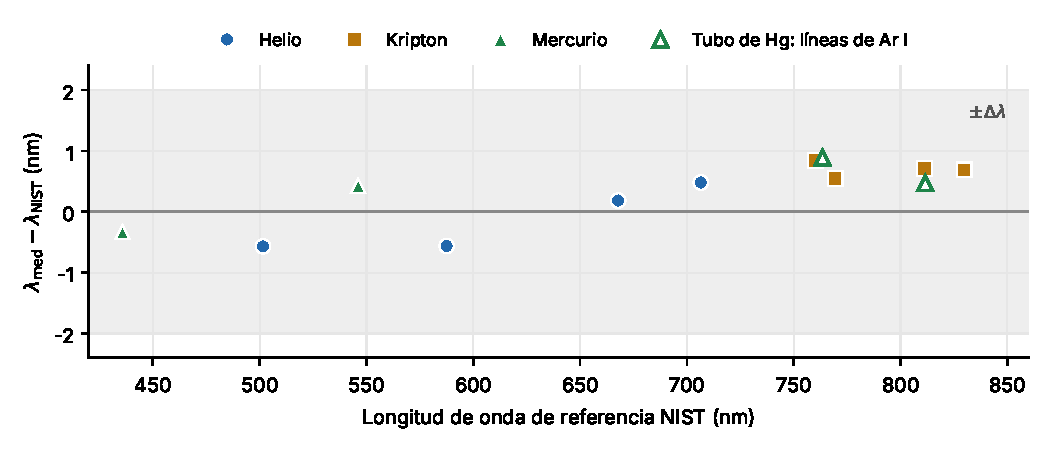
\includegraphics[width=0.92\textwidth]{residuos_conocidos.pdf}
\caption{Diferencia entre la longitud de onda medida y la del NIST para las líneas de la Tabla~\ref{tab:conocidos}. La franja gris indica la incertidumbre típica $\pm\Delta\lambda=\pm2\nm$.}
\label{fig:residuos}
\end{figure}

La Figura~\ref{fig:residuos} muestra que los residuos, además de ser pequeños, presentan una leve tendencia sistemática: son negativos en el extremo azul-verde (alrededor de $-0,5\nm$) y positivos en el rojo profundo e infrarrojo cercano (entre $+0,5$ y $+0,9\nm$). Un ajuste lineal de los residuos da una pendiente de unos $0,3\nm$ cada $100\nm$, lo que sugiere un pequeño error en la calibración en longitud de onda del espectrómetro. Este efecto es menor que la resolución del instrumento y no afecta la identificación de ninguna línea.

\subsection{Tubos incógnita}

Para los tubos incógnita en la planilla solo se registró el color observado y, en el N.º 1, la posición y el ancho de la banda. Las longitudes de onda de las líneas se obtuvieron a partir de las capturas del software (Anexo~\ref{anexo}): se calibraron los ejes de cada captura con su grilla (residuo de calibración menor que $0,4\nm$), se digitalizó la curva y se tomó como posición de cada línea el punto medio de su ancho a media altura. La incertidumbre de la digitalización ($\approx0,5\nm$) es menor que la resolución del espectrómetro, por lo que se mantuvo $\Delta\lambda=2\nm$. Los espectros digitalizados se muestran en la Figura~\ref{fig:incognitas}. Fuera de las regiones graficadas no se observó emisión en el rango de $350$ a $1000\nm$, salvo un pequeño pico de unas 20 cuentas cerca de $407\nm$ que aparece por igual en los espectros N.º 1 y N.º 3; al no depender del tubo, se lo atribuye al detector o a luz ambiente.

\begin{figure}[H]
\centering
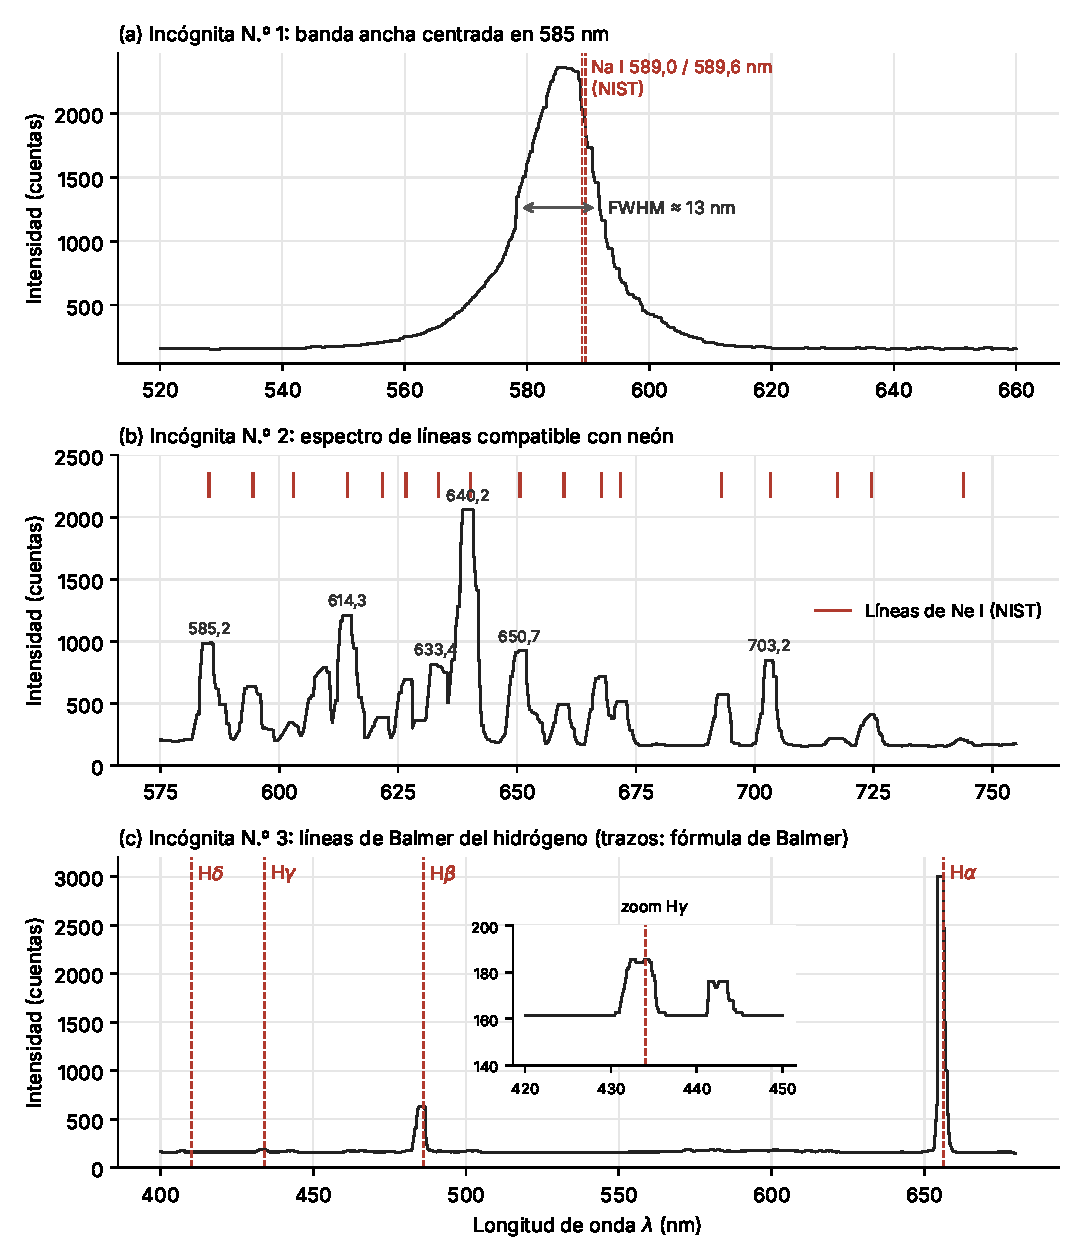
\includegraphics[width=0.93\textwidth]{espectros_incognita.pdf}
\caption{Espectros de los tubos incógnita, digitalizados a partir de las capturas del software, con las referencias del NIST \cite{nist-na,nist-ne} y las líneas de Balmer calculadas con la ecuación~\eqref{eq:rydberg} (en aire). En (b) se indica el valor de referencia de las líneas más intensas.}
\label{fig:incognitas}
\end{figure}

\subsubsection{Incógnita N.º 1: fuente no atómica (tipo LED)}

El espectro consiste en una única banda centrada en $\lambda=585\nm$, con un ancho a media altura de $13\nm$ (en la planilla se registró $\lambda=585\nm$ con $\Delta\lambda=15\nm$). Este espectro no es compatible con la emisión de un gas:
\begin{itemize}
    \item El ancho es unas cinco veces mayor que el de las líneas atómicas medidas con el mismo equipo ($\approx2$ a $2,5\nm$, limitado por el instrumento) y supera en más de tres órdenes de magnitud al ensanchamiento Doppler esperable para un gas.
    \item La única emisión atómica intensa en esa región sería el doblete D del sodio ($589,00$ y $589,59\nm$ \cite{nist-na}), cuyo centro queda $4\nm$ por encima del máximo medido. Además, una descarga de sodio mostraría el doblete infrarrojo del Na~I en $818,3$ y $819,5\nm$, donde no se observa señal por encima del ruido.
\end{itemize}
En cambio, el ancho medido coincide con el esperado para un LED según la ecuación \eqref{eq:anchoLED}: $\Delta\lambda\approx(585\nm)^2\cdot(46\ \mathrm{meV})/(1240\ \mathrm{eV\,nm})\approx13\nm$. Se concluye que la incógnita N.º 1 es una fuente de estado sólido de banda ancha, muy probablemente un LED amarillo-ámbar (típicamente de AlGaInP), en concordancia con la monocromaticidad observada a simple vista. Como no se trata de una línea atómica, no existe un ``valor real'' tabulado con el cual calcular el error porcentual.

\subsubsection{Incógnita N.º 2: neón}

El espectro presenta numerosas líneas entre $585$ y $745\nm$, sin emisión en el azul ni en el verde, lo que explica el color rojo-anaranjado observado. Las 17 líneas identificadas coinciden con líneas de Ne~I del NIST \cite{nist-ne}, como se detalla en la Tabla~\ref{tab:neon}.

\begin{table}[H]
\centering\small
\caption{Líneas de la incógnita N.º 2 ($\Delta\lambda=2\nm$) y su identificación con líneas de Ne~I (NIST, en aire).}
\label{tab:neon}
\begin{tabular}{@{}cccc@{\hspace{1.2cm}}cccc@{}}
\toprule
$\boldsymbol{\lambda}$ \textbf{(nm)} & \textbf{Ne I (nm)} & \textbf{Dif. (nm)} & \textbf{Error (\%)} &
$\boldsymbol{\lambda}$ \textbf{(nm)} & \textbf{Ne I (nm)} & \textbf{Dif. (nm)} & \textbf{Error (\%)}\\
\midrule
585,3 & 585,25 & $+0,05$ & 0,009 & 650,4 & 650,65 & $-0,25$ & 0,038\\
594,2 & 594,48 & $-0,28$ & 0,047 & 660,4 & 659,90 & $+0,50$ & 0,076\\
602,8 & 603,00 & $-0,20$ & 0,033 & 668,2 & 667,83 & $+0,37$ & 0,055\\
614,3 & 614,31 & $-0,01$ & 0,002 & 671,4 & 671,70 & $-0,30$ & 0,045\\
621,3 & 621,73 & $-0,43$ & 0,069 & 694,0 & 692,95 & $+1,05$ & 0,152\\
626,4 & 626,65 & $-0,25$ & 0,040 & 703,1 & 703,24 & $-0,14$ & 0,020\\
632,9 & 633,44 & $-0,54$ & 0,085 & 717,3 & 717,39 & $-0,09$ & 0,013\\
639,6 & 640,22 & $-0,62$ & 0,097 & 724,1 & 724,52 & $-0,42$ & 0,058\\
      &        &         &       & 743,6 & 743,89 & $-0,29$ & 0,039\\
\bottomrule
\end{tabular}
\end{table}

Las 17 líneas son compatibles con el neón (diferencia máxima de $1,05\nm$, error porcentual medio de $0,05\%$) y no queda ninguna línea intensa sin identificar. El pico en torno a $608,5\nm$ no se incluyó en la tabla porque corresponde a dos líneas de Ne~I ($607,43$ y $609,62\nm$) separadas por apenas $2,2\nm$, que el espectrómetro no resuelve. Las intensidades relativas medidas no coinciden con las del NIST, donde las líneas más intensas son la de $692,9\nm$ (1000) y las de $703,2$, $717,4$ y $724,5\nm$ (800), mientras que aquí domina la de $640,2\nm$ (200 en el NIST). Esto es esperable, ya que las intensidades dependen de las condiciones de la descarga (presión y corriente) y de la respuesta espectral del espectrómetro; por eso la identificación se basa en las longitudes de onda. Se concluye que la incógnita N.º 2 es un tubo de \textbf{neón}.

\subsubsection{Incógnita N.º 3: hidrógeno}

El espectro muestra una línea muy intensa en $655,5\nm$ y otra más débil en $485,9\nm$, que coinciden con H$\alpha$ y H$\beta$ de la serie de Balmer. La combinación de una línea roja y una azul explica el color rosado-violáceo del tubo, registrado como ``rojo y azul'' en la planilla. Se observa además un pico débil centrado en $433,4\nm$ (unas 25 cuentas sobre el fondo, ausente en los otros dos espectros), compatible con H$\gamma$. Como en esa zona hay otras fluctuaciones del fondo de amplitud comparable (por ejemplo, cerca de $442\nm$), esta identificación se considera tentativa. H$\delta$ ($410,2\nm$) no se detecta, lo que es razonable dada la menor intensidad de las líneas superiores de la serie y la menor sensibilidad del detector en el violeta. Se concluye que la incógnita N.º 3 es un tubo de \textbf{hidrógeno}; la comparación cuantitativa se presenta a continuación.

\subsection{Series de Balmer y Lyman}

Con la ecuación \eqref{eq:rydberg} y el valor de $R_H$ de la ecuación \eqref{eq:RH} se calcularon las primeras líneas de ambas series. Por ejemplo, para H$\alpha$,
\begin{equation*}
    \lambda_{\mathrm{vac}}=\left[R_H\left(\frac{1}{2^2}-\frac{1}{3^2}\right)\right]^{-1}=\frac{36}{5R_H}=656,47\nm,
    \qquad
    \lambda_{\mathrm{aire}}=\frac{656,47\nm}{1,000276}=656,29\nm.
\end{equation*}

\begin{table}[H]
\centering\small
\caption{Serie de Balmer ($n_f=2$): valores calculados, valores del NIST \cite{nist-h} y valores medidos en la incógnita N.º 3. El error se calcula respecto del valor teórico en aire.}
\label{tab:balmer}
\begin{tabular}{@{}lcccccc@{}}
\toprule
\textbf{Línea} & $\boldsymbol{n_i}$ & $\boldsymbol{\lambda_{\mathrm{vac}}}$ \textbf{teórica (nm)} & $\boldsymbol{\lambda_{\mathrm{aire}}}$ \textbf{teórica (nm)} & \textbf{NIST (nm)} & \textbf{Medida (nm)} & \textbf{Error (\%)}\\
\midrule
H$\alpha$   & 3 & 656,47 & 656,29 & 656,28 & $655,5\pm2$ & 0,120\\
H$\beta$    & 4 & 486,27 & 486,14 & 486,13 & $485,9\pm2$ & 0,049\\
H$\gamma$   & 5 & 434,17 & 434,05 & 434,05 & $433,4\pm2$\,$^{*}$ & 0,150\\
H$\delta$   & 6 & 410,29 & 410,18 & 410,17 & no detectada & --\\
H$\varepsilon$ & 7 & 397,12 & 397,01 & 397,01 & no detectada & --\\
Límite      & $\infty$ & 364,71 & 364,60 & -- & -- & --\\
\bottomrule
\multicolumn{7}{@{}l}{\footnotesize $^{*}$ Identificación tentativa (señal débil).}
\end{tabular}
\end{table}

\begin{table}[H]
\centering\small
\caption{Serie de Lyman ($n_f=1$): longitudes de onda teóricas en el vacío.}
\label{tab:lyman}
\begin{tabular}{@{}lccccc@{}}
\toprule
\textbf{Línea} & Ly$\alpha$ & Ly$\beta$ & Ly$\gamma$ & Ly$\delta$ & Límite\\
\midrule
$n_i$ & 2 & 3 & 4 & 5 & $\infty$\\
$\lambda_{\mathrm{vac}}$ (nm) & 121,57 & 102,57 & 97,25 & 94,97 & 91,18\\
\bottomrule
\end{tabular}
\end{table}

Los valores teóricos de la serie de Balmer reproducen los del NIST con diferencias menores a $0,01\nm$, y las tres líneas observadas coinciden con ellos dentro de $\Delta\lambda$, con errores porcentuales de entre $0,05$ y $0,15\%$. La serie de Lyman, en cambio, cae íntegramente en el ultravioleta de vacío ($91$ a $122\nm$). Esa radiación es absorbida por el vidrio del tubo y por el oxígeno del aire, y además está muy por debajo del límite inferior del espectrómetro ($350\nm$), por lo que no puede observarse con este montaje. Su comparación con el espectro obtenido es entonces negativa: no aparece ninguna línea de Lyman, tal como se espera.

\textbf{Constante de Rydberg experimental.} Invirtiendo la ecuación \eqref{eq:rydberg} para las líneas medidas (convertidas previamente al vacío) se obtiene
\begin{equation}
    R_{\mathrm{exp}}=\frac{1}{\lambda_{\mathrm{vac}}\left(\dfrac{1}{4}-\dfrac{1}{n_i^2}\right)},
    \qquad
    \frac{\Delta R}{R}=\frac{\Delta\lambda}{\lambda}.
\end{equation}
Con H$\alpha$ resulta $R=(1,0981\pm0,0034)\times10^{7}\ \mathrm{m^{-1}}$ y con H$\beta$, $R=(1,0973\pm0,0045)\times10^{7}\ \mathrm{m^{-1}}$. El promedio ponderado por $1/(\Delta R)^2$ es
\begin{equation}
    R_{\mathrm{exp}}=(1,0978\pm0,0027)\times10^{7}\ \mathrm{m^{-1}},
\end{equation}
que difiere del valor teórico $R_H=1,09678\times10^{7}\ \mathrm{m^{-1}}$ en un $0,09\%$, muy por debajo de la incertidumbre relativa ($0,25\%$). La línea H$\gamma$ no se incluyó en este cálculo por ser tentativa.

\subsection{Resumen de los tubos incógnita}

\begin{table}[H]
\centering\small
\caption{Resultado para los tubos incógnita en el formato de la consigna.}
\label{tab:incognitas}
\begin{tabular}{@{}cllcccc@{}}
\toprule
\textbf{Tubo} & \textbf{Color} & \textbf{Identificación} & $\boldsymbol{\lambda}$ \textbf{(nm)} & $\boldsymbol{\Delta\lambda}$ \textbf{(nm)} & \textbf{Valor real (nm)} & \textbf{Error (\%)}\\
\midrule
N.º 1 & Amarillo & Fuente de estado sólido (LED) & 585 & 15 & -- & --\\
\midrule
\multirow{3}{*}{N.º 2} & \multirow{3}{*}{Varios rojos} & \multirow{3}{*}{Neón (17 líneas, Tabla~\ref{tab:neon})} & 585,3 & 2 & 585,25 & 0,009\\
 & & & 639,6 & 2 & 640,22 & 0,097\\
 & & & 703,1 & 2 & 703,24 & 0,020\\
\midrule
\multirow{3}{*}{N.º 3} & \multirow{3}{*}{Rojo y azul} & \multirow{3}{*}{Hidrógeno (serie de Balmer)} & 655,5 & 2 & 656,28 & 0,119\\
 & & & 485,9 & 2 & 486,13 & 0,047\\
 & & & 433,4 & 2 & 434,05 & 0,150\\
\bottomrule
\end{tabular}
\end{table}

%=====================================================================
\section{Análisis de los resultados obtenidos}

\subsection{Exactitud del espectrómetro}

Las 12 líneas de los gases conocidos, las 17 del neón y las 3 del hidrógeno coinciden con sus valores de referencia dentro de la incertidumbre instrumental, con errores porcentuales menores al $0,2\%$. Esto confirma que el espectrómetro estaba correctamente calibrado y que la principal limitación de la medición es su resolución ($\approx2\nm$), no su exactitud. La leve tendencia de los residuos con la longitud de onda (Figura~\ref{fig:residuos}) podría corregirse recalibrando el equipo con una lámpara patrón de líneas bien conocidas, como la misma de Hg-Ar.

\subsection{Fuentes de error}

\begin{itemize}
    \item \textbf{Resolución finita:} líneas separadas por menos de $\sim2\nm$ aparecen como un único pico (tripletes del He, Kr~I 810,4/811,3~nm, Ar~I 810,4/811,5~nm y Ne~I 607,4/609,6~nm), cuyo máximo puede quedar corrido respecto de la componente tomada como referencia.
    \item \textbf{Lectura del máximo con el cursor:} la posición del cursor y la discretización en píxeles del detector introducen una incertidumbre del orden de $0,5\nm$.
    \item \textbf{Saturación e intensidad:} un pico saturado presenta un máximo plano y mal definido; por esta razón se ajustó la posición de la fibra. Las líneas muy débiles, como H$\gamma$, quedan cerca del nivel de ruido.
    \item \textbf{Calibración en longitud de onda:} produce un corrimiento sistemático de algunas décimas de nanómetro que varía con $\lambda$.
    \item \textbf{Composición real del tubo:} gases de llenado (como el Ar del tubo de Hg) o impurezas agregan líneas que no pertenecen al elemento nominal. Para identificar un tubo deben compararse \emph{todas} sus líneas con las bases de datos, y no solo las del visible.
    \item \textbf{Digitalización de las capturas} (solo incógnitas): calibración de los ejes ($<0,4\nm$) y ancho de píxel de la pantalla original ($\approx1\nm$).
\end{itemize}

\subsection{Conclusión}

Se midieron los espectros de emisión de helio, kriptón y mercurio con un espectrómetro de red de difracción, y todas las líneas coincidieron con los valores del NIST con errores menores al $0,12\%$, dentro de la resolución del instrumento. La verificación con la base de datos mostró que las líneas infrarrojas del tubo de kriptón pertenecen al Kr~I, mientras que las dos líneas anómalas del tubo de mercurio (764,4 y 812,0~nm) corresponden al argón usado como gas de llenado. A partir de sus espectros se identificaron dos de los tubos incógnita como \textbf{neón} (17 líneas) e \textbf{hidrógeno} (serie de Balmer). El tercero no es un gas: su banda de $13\nm$ de ancho centrada en $585\nm$ corresponde a una fuente de estado sólido tipo LED. Las fórmulas de Balmer reprodujeron las líneas observadas del hidrógeno con errores de entre $0,05$ y $0,15\%$ y permitieron obtener $R_{\mathrm{exp}}=(1,0978\pm0,0027)\times10^{7}\ \mathrm{m^{-1}}$, en excelente acuerdo con el valor teórico. Las líneas de Lyman, en el ultravioleta de vacío, quedan fuera del alcance del montaje.

%=====================================================================
\section{Referencias}
\begingroup
\renewcommand{\section}[2]{}
\begin{thebibliography}{99}
\bibitem{consigna} Cátedra de Física IV, ITBA. \emph{Espectrometría} (guía de trabajos prácticos de laboratorio).

\bibitem{nist-handbook} J.~E.~Sansonetti y W.~C.~Martin, ``Handbook of Basic Atomic Spectroscopic Data'', \emph{J. Phys. Chem. Ref. Data} \textbf{34}, 1559 (2005). Versión en línea (NIST): \url{https://physics.nist.gov/PhysRefData/Handbook/index.html}

\bibitem{nist-he} NIST, \emph{Strong Lines of Helium (He)}: \url{https://physics.nist.gov/PhysRefData/Handbook/Tables/heliumtable2.htm}

\bibitem{nist-kr} NIST, \emph{Strong Lines of Krypton (Kr)}: \url{https://physics.nist.gov/PhysRefData/Handbook/Tables/kryptontable2.htm}

\bibitem{nist-hg} NIST, \emph{Strong Lines of Mercury (Hg)}: \url{https://physics.nist.gov/PhysRefData/Handbook/Tables/mercurytable2.htm}

\bibitem{nist-ar} NIST, \emph{Strong Lines of Argon (Ar)}: \url{https://physics.nist.gov/PhysRefData/Handbook/Tables/argontable2.htm}

\bibitem{nist-ne} NIST, \emph{Strong Lines of Neon (Ne)}: \url{https://physics.nist.gov/PhysRefData/Handbook/Tables/neontable2.htm}

\bibitem{nist-h} NIST, \emph{Strong Lines of Hydrogen (H)}: \url{https://physics.nist.gov/PhysRefData/Handbook/Tables/hydrogentable2.htm}

\bibitem{nist-na} NIST, \emph{Strong Lines of Sodium (Na)}: \url{https://physics.nist.gov/PhysRefData/Handbook/Tables/sodiumtable2.htm}

\bibitem{codata} E.~Tiesinga, P.~J.~Mohr, D.~B.~Newell y B.~N.~Taylor, ``CODATA recommended values of the fundamental physical constants: 2018'', \emph{Rev. Mod. Phys.} \textbf{93}, 025010 (2021). \url{https://physics.nist.gov/cuu/Constants/}

\bibitem{morton} D.~C.~Morton, ``Atomic data for resonance absorption lines. II. Wavelengths longward of the Lyman limit for heavy elements'', \emph{Astrophys. J. Suppl. Ser.} \textbf{130}, 403 (2000).

\bibitem{schubert} E.~F.~Schubert, \emph{Light-Emitting Diodes}, 2.ª ed., Cambridge University Press (2006), cap.~5.

\bibitem{eisberg} R.~Eisberg y R.~Resnick, \emph{Física cuántica: átomos, moléculas, sólidos, núcleos y partículas}, Limusa (1978), cap.~4.

\bibitem{hecht} E.~Hecht, \emph{Óptica}, 3.ª ed., Addison-Wesley (2000), cap.~10.
\end{thebibliography}
\endgroup

%=====================================================================
\appendix
\section{Anexo: capturas de los espectros de los tubos incógnita}
\label{anexo}

\begin{figure}[H]
\centering
\begin{subfigure}{0.49\textwidth}\centering
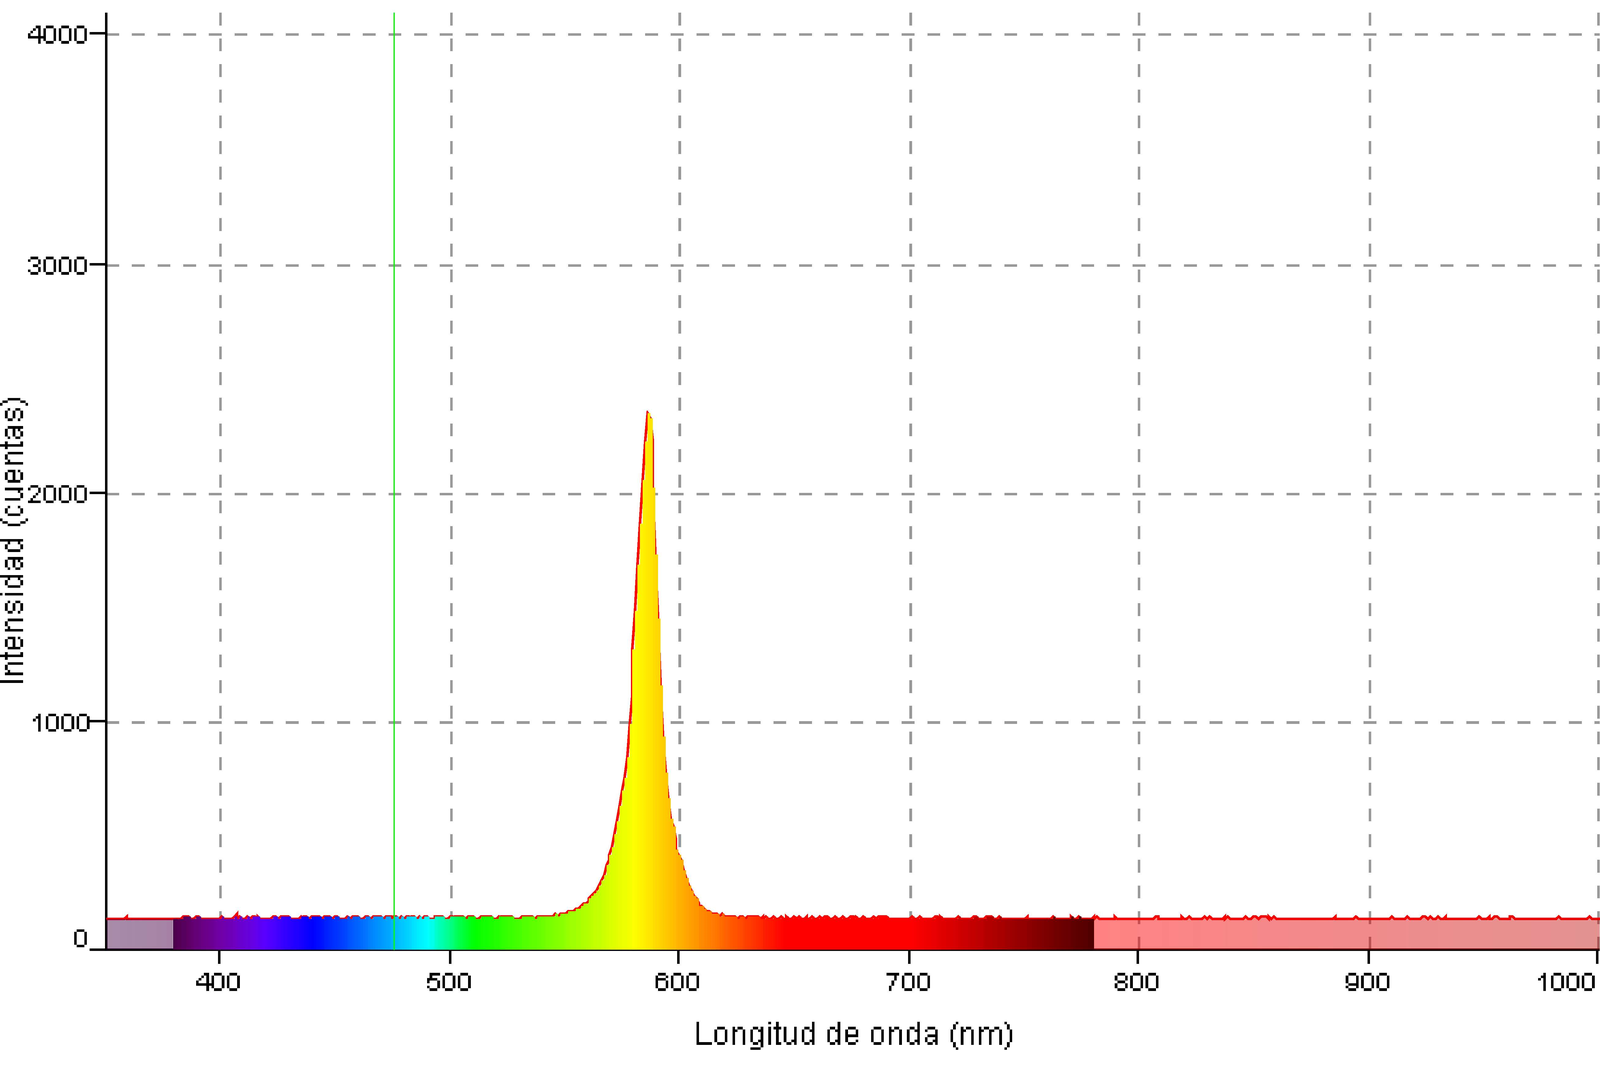
\includegraphics[width=\textwidth]{captura_N1.png}
\caption{Incógnita N.º 1}
\end{subfigure}\hfill
\begin{subfigure}{0.49\textwidth}\centering
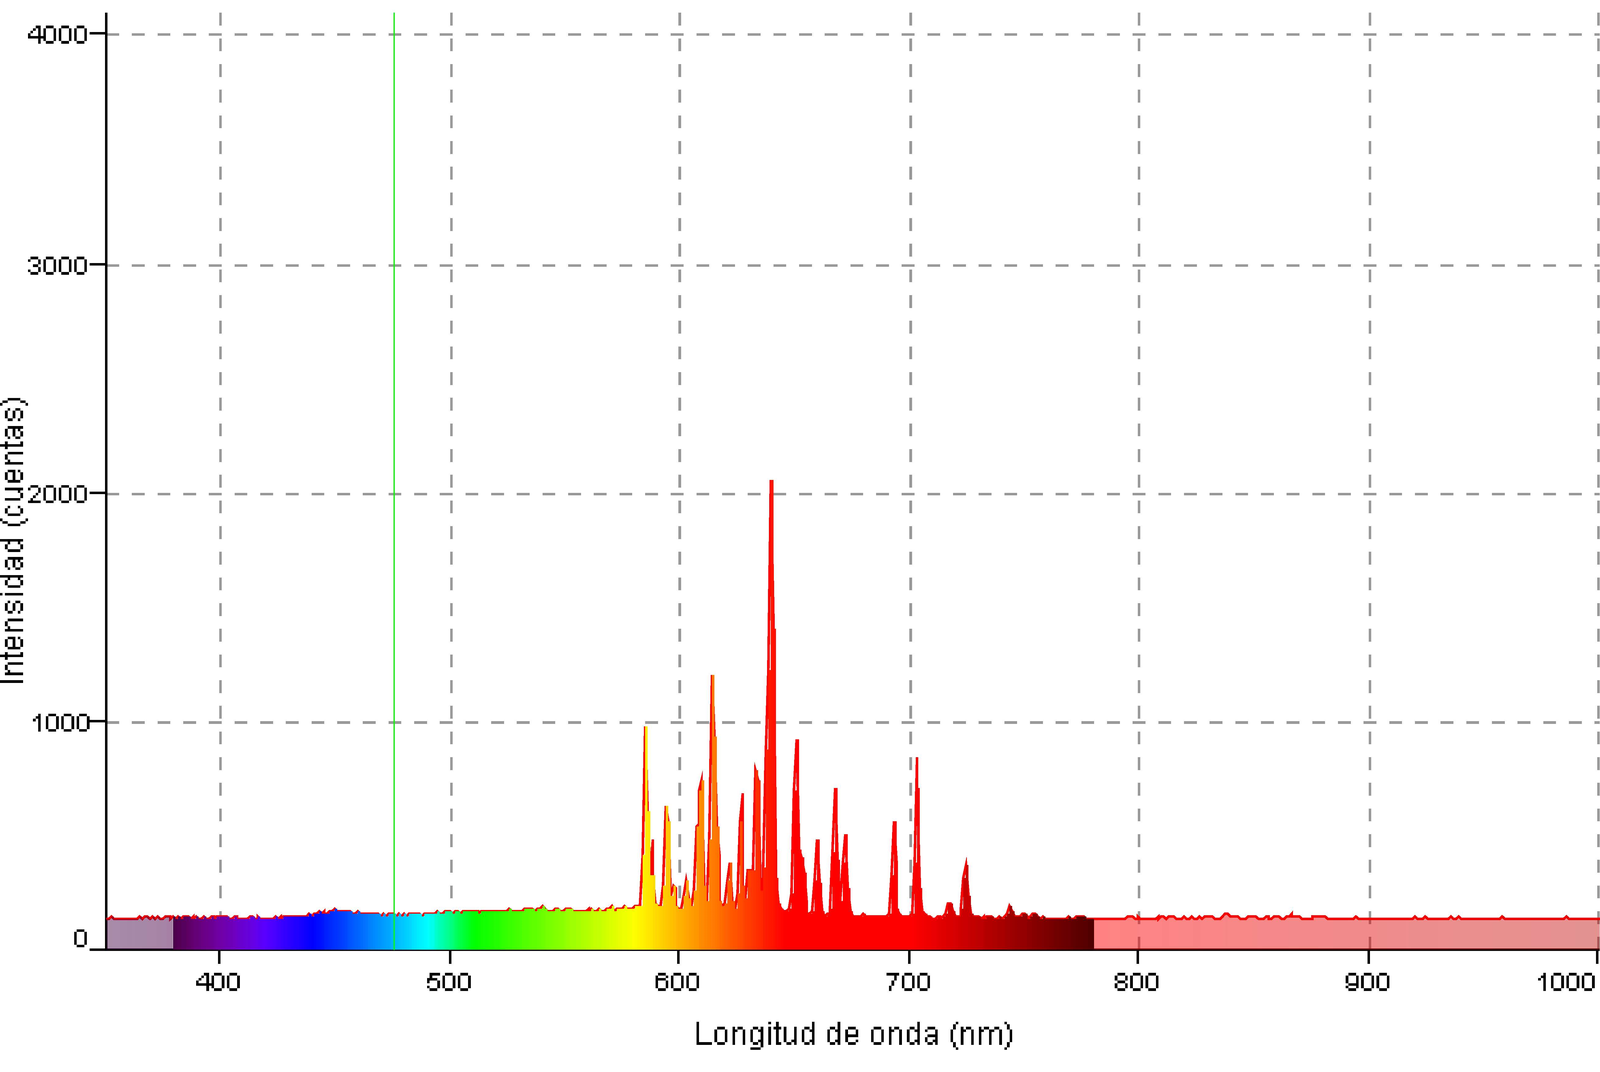
\includegraphics[width=\textwidth]{captura_N2.png}
\caption{Incógnita N.º 2}
\end{subfigure}

\vspace{0.4em}
\begin{subfigure}{0.49\textwidth}\centering
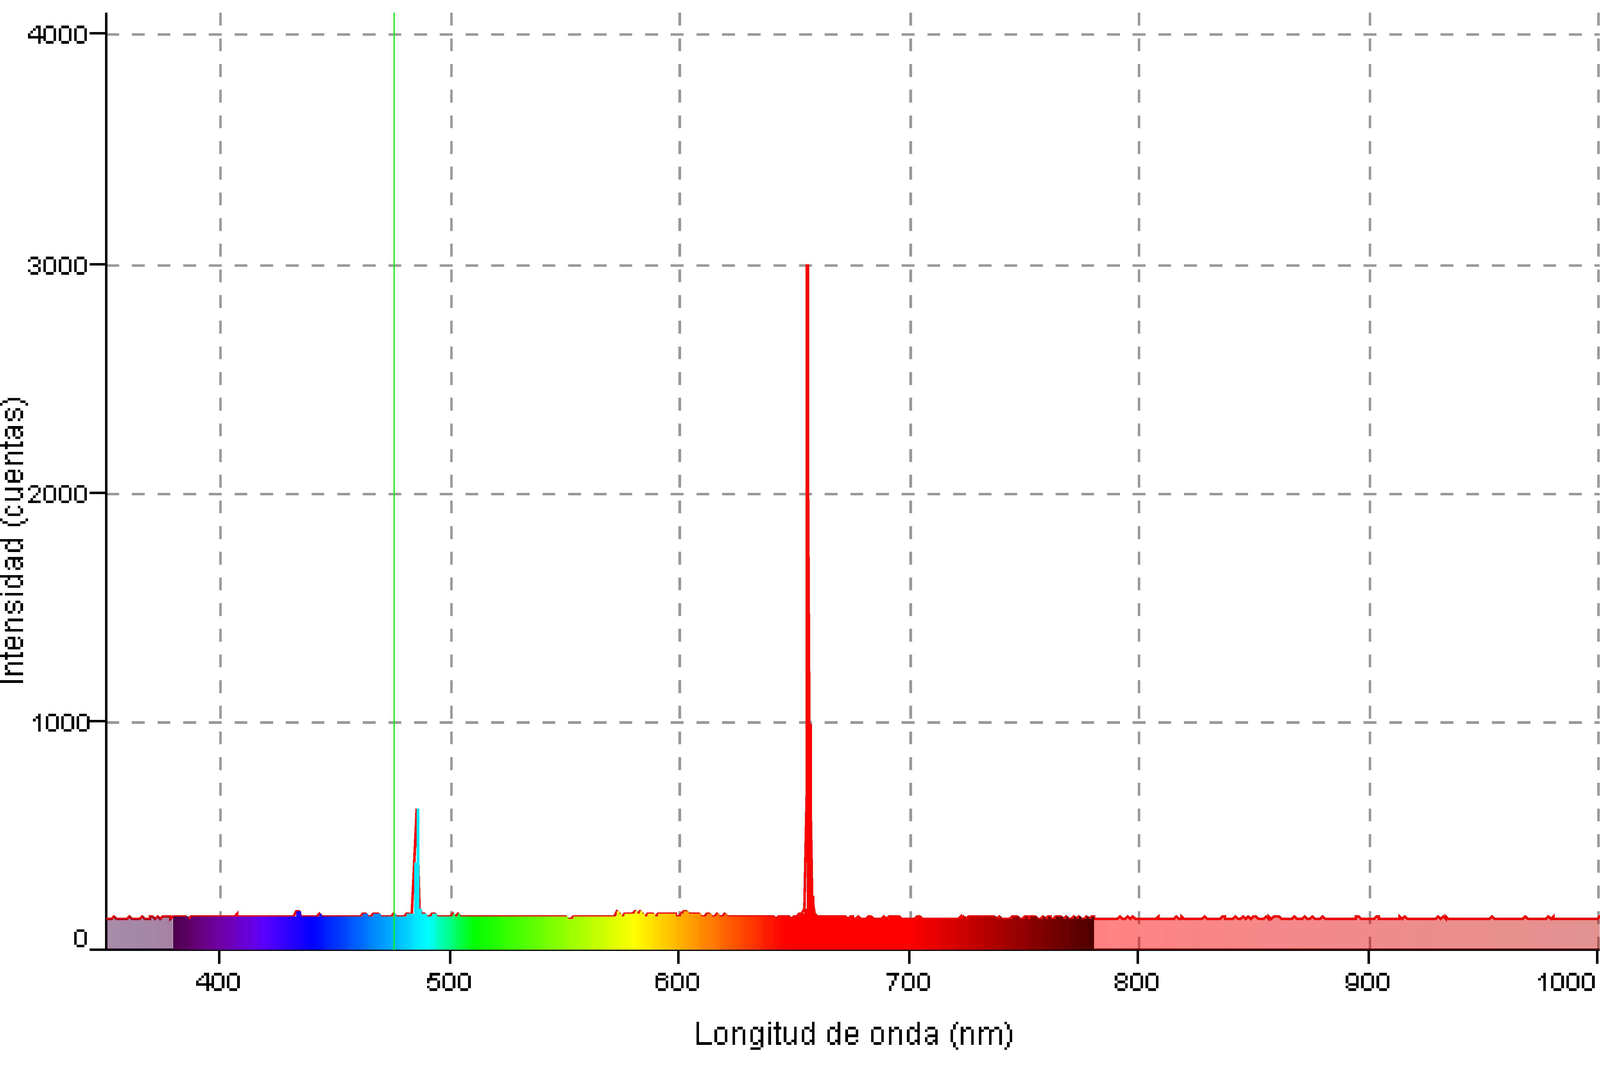
\includegraphics[width=\textwidth]{captura_N3.png}
\caption{Incógnita N.º 3}
\end{subfigure}
\caption{Capturas originales del software del espectrómetro (archivos \texttt{Gas-desconocidoN1.pdf} a \texttt{Gas-desconocidoN3.pdf}). La línea vertical verde en $\approx475\nm$ es el cursor del programa.}
\label{fig:capturas}
\end{figure}

\end{document}
